\documentclass[12pt]{article}
\usepackage{amsmath,amsfonts,amsthm,amssymb}
\usepackage{setspace}
\usepackage{fancyhdr}
\usepackage{lastpage}
\usepackage{extramarks}
\usepackage[ruled,vlined]{algorithm2e}
\usepackage{chngpage}
\usepackage{soul,color}
\usepackage{hyperref}
\usepackage{graphicx,float,wrapfig}
\usepackage{ listings}

\graphicspath{ {../images/}}

\newcommand{\Class}{ \normalsize CS 395T: Robot Learning (Fall 2017)}

%\newcommand{\ClassInstructor}{Fares}
% Homework Specific Information. Change it to your own
\newcommand{\Title}{Assignment 1}
\newcommand{\DueDate}{Wednesday, September 20, by 11:59pm}
\newcommand{\StudentName}{Sean Kirmani}
\newcommand{\StudentClass}{51920}
\newcommand{\StudentNumber}{sk35375}
\newcommand{\complexityclass}[1]{\textsc{#1}}
\newcommand{\ccp}{\complexityclass{P}}
\newcommand{\ccnp}{\complexityclass{NP}}
% In case you need to adjust margins:
\topmargin=-0.45in      %
\evensidemargin=0in     %
\oddsidemargin=0in      %
\textwidth=6.5in        %
\textheight=9.0in       %
\headsep=0.25in         %

% Setup the header and footer
\pagestyle{fancy}                                                       %
\lhead{\StudentName}                                                 %
\chead{\Title}  %
\rhead{\firstxmark}                                                     %
\lfoot{\lastxmark}                                                      %
\cfoot{}                                                                %
\rfoot{Page\ \thepage\ of\ \protect\pageref{LastPage}}                          %
\renewcommand\headrulewidth{0.4pt}                                      %
\renewcommand\footrulewidth{0.4pt}                                      %

%%%%%%%%%%%%%%%%%%%%%%%%%%%%%%%%%%%%%%%%%%%%%%%%%%%%%%%%%%%%%
% Some tools
\newcommand{\enterProblemHeader}[1]{\nobreak\extramarks{#1}{#1 continued on next page\ldots}\nobreak%
	\nobreak\extramarks{#1 (continued)}{#1 continued on next page\ldots}\nobreak}%
\newcommand{\exitProblemHeader}[1]{\nobreak\extramarks{#1 (continued)}{#1 continued on next page\ldots}\nobreak%
	\nobreak\extramarks{#1}{}\nobreak}%

\newcommand{\homeworkProblemName}{}%
\newcounter{homeworkProblemCounter}%
\newenvironment{homeworkProblem}[1][Problem \arabic{homeworkProblemCounter}]%
{\stepcounter{homeworkProblemCounter}%
	\renewcommand{\homeworkProblemName}{#1}%
	\section*{\homeworkProblemName}%
	\enterProblemHeader{\homeworkProblemName}}%
{\exitProblemHeader{\homeworkProblemName}}%

\newcommand{\homeworkSectionName}{}%
\newlength{\homeworkSectionLabelLength}{}%
\newenvironment{homeworkSection}[1]%
{% We put this space here to make sure we're not connected to the above.
	
	\renewcommand{\homeworkSectionName}{#1}%
	\settowidth{\homeworkSectionLabelLength}{\homeworkSectionName}%
	\addtolength{\homeworkSectionLabelLength}{0.25in}%
	\changetext{}{-\homeworkSectionLabelLength}{}{}{}%
	\subsection*{\homeworkSectionName}%
	\enterProblemHeader{\homeworkProblemName\ [\homeworkSectionName]}}%
{\enterProblemHeader{\homeworkProblemName}%
	
	% We put the blank space above in order to make sure this margin
	% change doesn't happen too soon.
	\changetext{}{+\homeworkSectionLabelLength}{}{}{}}%

\newcommand{\Answer}{\ \\\textbf{Answer:} }
\newcommand{\Acknowledgement}[1]{\ \\{\bf Acknowledgement:} #1}

%%%%%%%%%%%%%%%%%%%%%%%%%%%%%%%%%%%%%%%%%%%%%%%%%%%%%%%%%%%%%


%%%%%%%%%%%%%%%%%%%%%%%%%%%%%%%%%%%%%%%%%%%%%%%%%%%%%%%%%%%%%
% Make title
\title{\textmd{\bf \Class\\ \Title}\\\vspace{0.1in}\small{Due\ on\ \DueDate}}
\date{}
\author{\textbf{\StudentName}\ \ \StudentClass\ \ \StudentNumber}
%%%%%%%%%%%%%%%%%%%%%%%%%%%%%%%%%%%%%%%%%%%%%%%%%%%%%%%%%%%%%

\begin{document}
\maketitle \thispagestyle{empty}
% Begin edit from here

In this assignment, we implemented Dynamic Movement Primitives, or DMPs. A DMP can learn, generalize, and improve given tasks. We simplified the representation for the 2D domain, but on a robot, we have significantly more degrees of freedom. Both DMPs learn independently, but are linked by the phase variable. \\

We demonstrate cartesian DMP learning and planning. When given a single demonstration input, we simply save the demonstration's keypoints and linearly interpolate between them. Theoretically, we could smooth even further with spline interpolation, but that was out of scope of this implementation. As soon as we are given a second demonstration, we stop using linear demonstrations, and then use a regression to approximate $f(s)$. \\

For our demonstration input, we pass in a sine motion. Below we display the ground truth input demonstration we are trying to learn as blue in all of our examples, and our planned trajectory path with red. We visualize the actual path taken as well as the individual position of x and y over time. \\

Below we see our system reconstruct the trajectory it had just learned with one input. Since we only have one input, we are planning by linearly interpolating between the points. We replay the same trajectory with the same start and goal position as the demonstration over the same length of time in seconds.

\begin{center}
	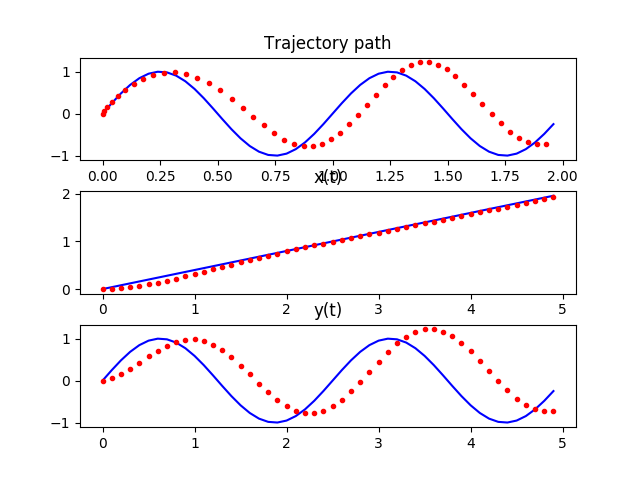
\includegraphics[width=0.7\textwidth]{linear_demonstration}
\end{center}

It does seem like we experience some phase lag since our initial acceleration is 0.  \\

We show that we can generalize to new start and goal points below, thus we have learned some spatially independent policy.

\begin{center}
	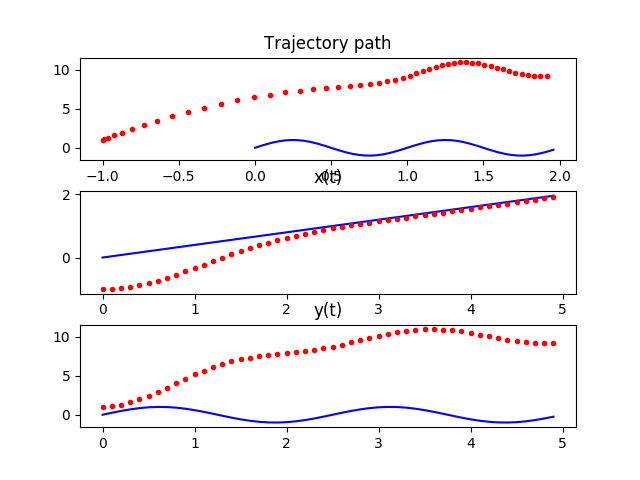
\includegraphics[width=0.7\textwidth]{linear_generalization_spatial}
\end{center}

Above we see that we are going from $[-1, 0]$ to $[2, 10]$, which is a fairly vertical path. We see the sine wave motion from our path from the start to the end. \\

We prove that we can also generalize over time trivially. Below we show the same trajectory being demonstrated at both double-speed as well as half-speed.

\begin{center}
	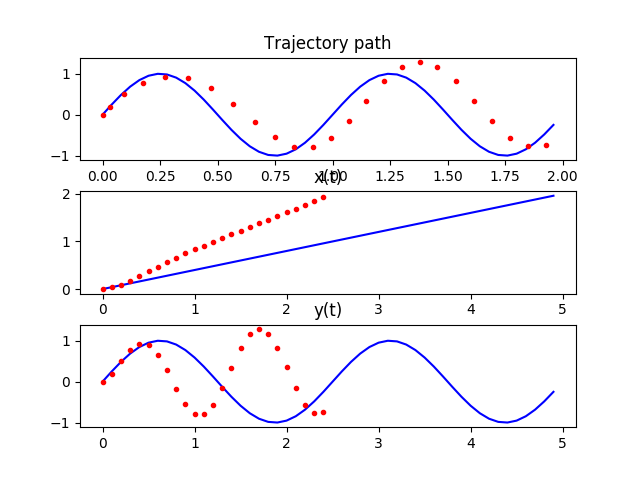
\includegraphics[width=0.4\textwidth]{linear_generalization_double_speed}
	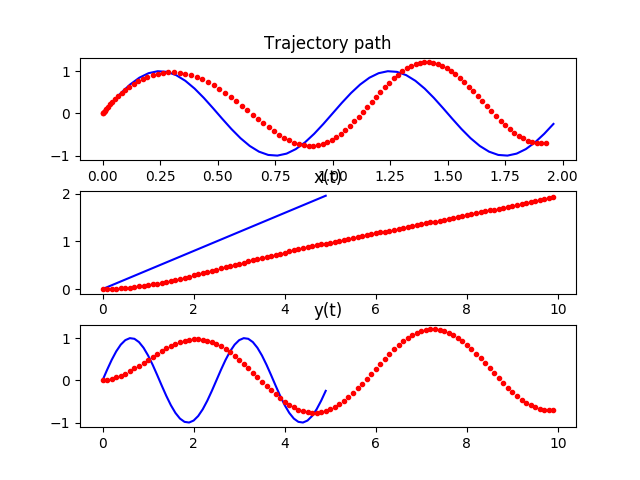
\includegraphics[width=0.4\textwidth]{linear_generalization_half_speed}
\end{center}

So far, we have shown our system outputs generalization capabilities using only our linear interpolation from one example. To be a bit fancy, I used a neural net for regression instead of an RBF kernel regression which I implemented with Tensorflow. \\

To test our systems ability to regress with multiple examples, we can create a new input demonstration with some noise, like the one visualized below.

\begin{center}
	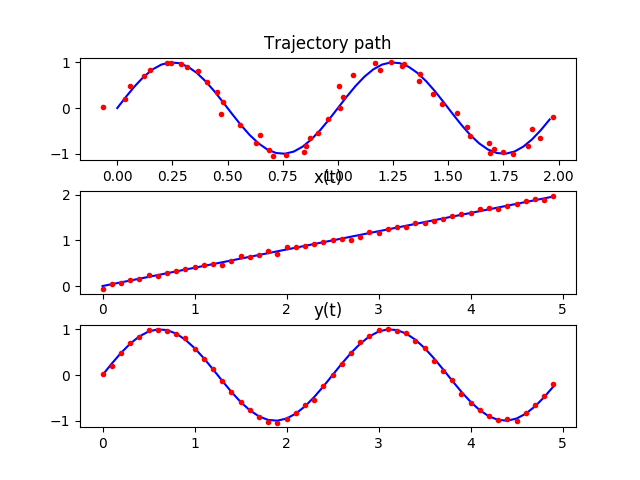
\includegraphics[width=0.7\textwidth]{noisy_demonstration}
\end{center}

We can train our regression based the original demonstration and this noisy generation and see what our system learned from multiple examples. On the left, we have our original linear interpolation from the first example and on the right we have our output learned from two demonstrations.

\begin{center}
	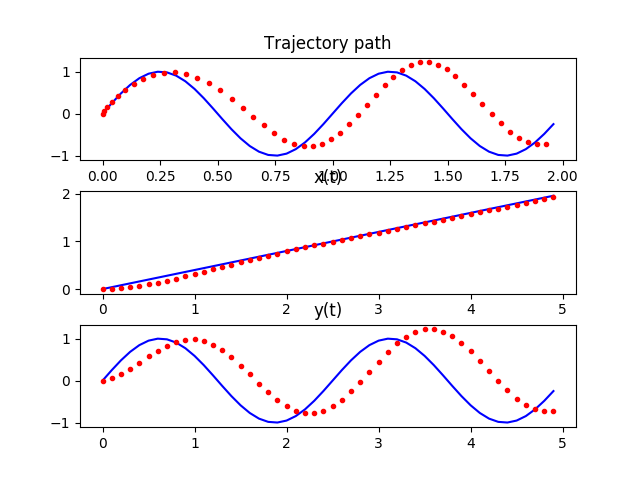
\includegraphics[width=0.4\textwidth]{linear_demonstration}
	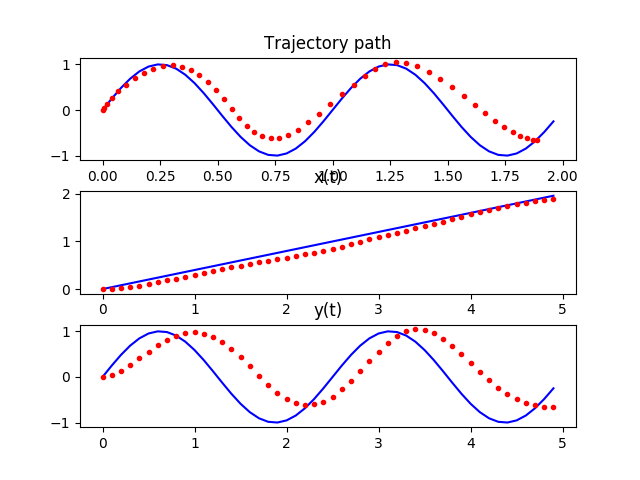
\includegraphics[width=0.4\textwidth]{regression_demonstration}
\end{center}

We qualitatively can see that we can pretty closely approximate our function with a regression. It seems pretty successful from only two examples. Given many noisy demonstrations, we would ideally converge toward the desired motion path. \\

We also want to make sure that generalization still holds with multiple examples. Below I compare the side-by-side view of our system generalizing to a new start and end goal. On the left we show our previous generalization with the linear interpolation, and on the right we are attempting to generalize a path using a regression.

\begin{center}
	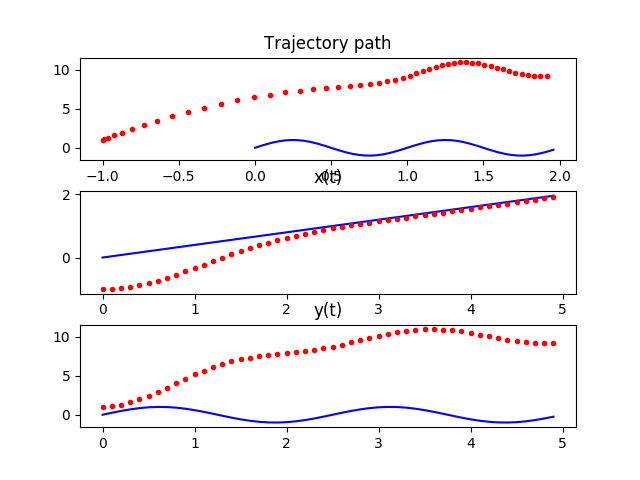
\includegraphics[width=0.4\textwidth]{linear_generalization_spatial}
	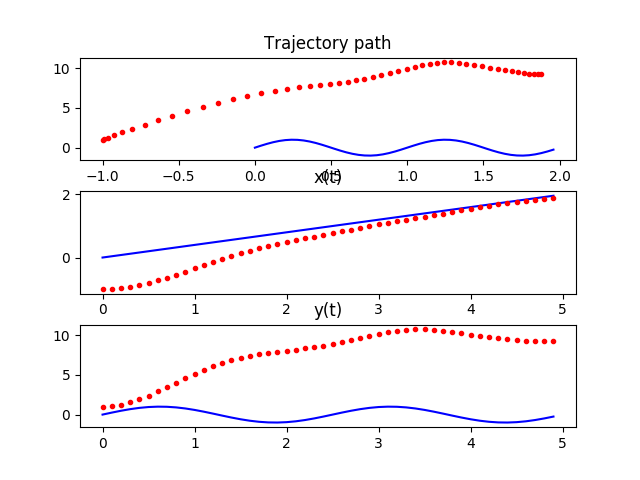
\includegraphics[width=0.4\textwidth]{regression_generalization_spatial}
\end{center}

Finally, we add a coupling term to verify that we can avoid obstacles. We feel some force away in the direction away from the object with a gaussian strength that weakens with distance. We plan our path around these obstacles. Below we show how our system handles obstacles, both when using linear interpolation (left) and regression (right) for function approximation.

\begin{center}
	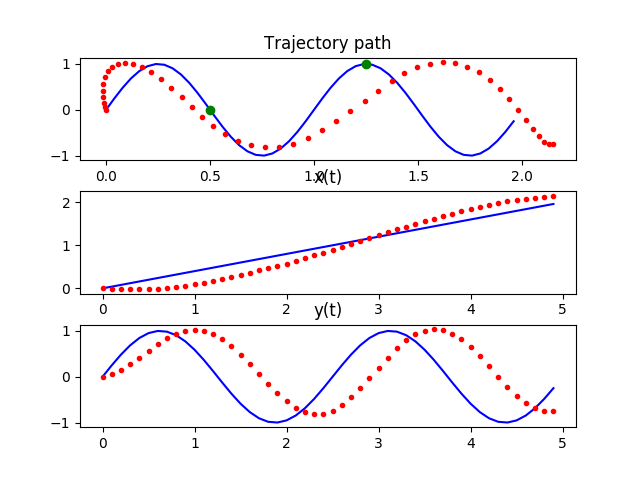
\includegraphics[width=0.4\textwidth]{linear_obstacle_avoidance_1}
	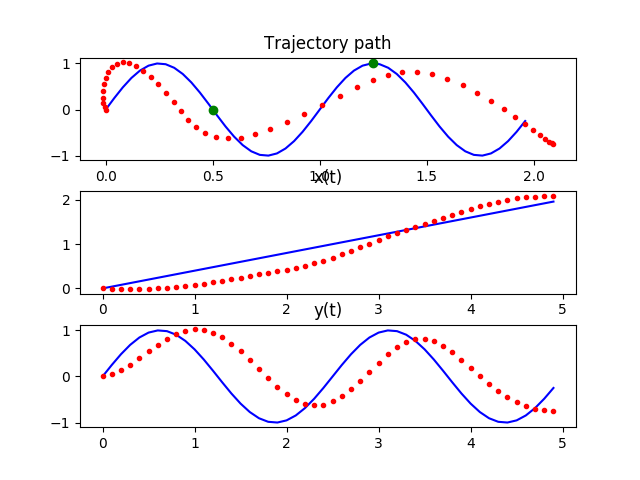
\includegraphics[width=0.4\textwidth]{regression_obstacle_avoidance_1}
	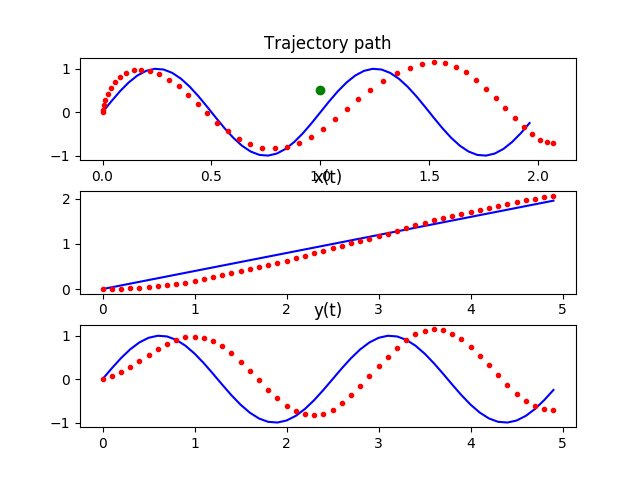
\includegraphics[width=0.4\textwidth]{linear_obstacle_avoidance_2}
	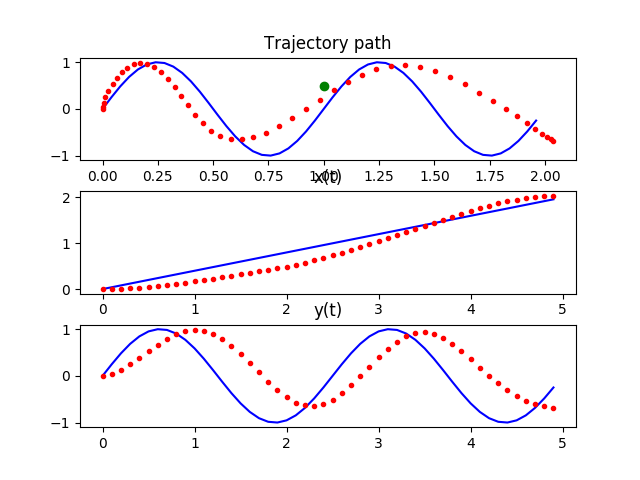
\includegraphics[width=0.4\textwidth]{regression_obstacle_avoidance_2}
\end{center}

With object avoidance, we still maintain the ``waviness" of the path but we feel a force that pushes us away from objects. Our motion is still smooth, which is a nice benefit we get from using the set of differential equations to model our trajectory. \\

Additional questions:
\begin{enumerate}
	\item It seems our system generalizes properly to new starts and goals pretty well if we don't have a path that deviates too much. However, our representation can be considered ill-defined, because when we want to represent our curve in a path that is perpendicular to our representation, we would probably expect a wave, but rotated from a top-down perspective. There seems to be ambiguity in our expected motion given rotations about our start and end point. The direction vector seems to matter.
	\item Since our DMP is representing by a differential equations, we would be able to compute our desired $\dot{v}$ in real-time so that we can be robust to moving objects and other unexpected dynamics such as moving obstacles or unexpected perturbation. This seems nice because we have robustness to unexpected dynamics if our plan fails or seems to not be converging to 0.
	\item We have several free parameters to optimize against. We have $K$ which represents our spring constant. We have $\alpha$ which represents our convergence speed. We have $\beta$ which defines the decay speed of our Gaussian force for objects, and $\gamma$ which scales those amplitudes. Then in our regression, we may have some hyper-parameters to optimize as well depending our our learning method.
\end{enumerate}

\end{document}
